% !TeX root=debugging.tex

\section{What \& Why}

\subsection{Bug}

\begin{frame}
    \frametitle{What is \textit{bug}?}
    \onslide<1-1>
    \tikz[overlay]\node[rotate=-6] at (60ex,8ex) {
\includegraphics[width=0.25\textwidth]{wikipedia.png}};
    \onslide<1->
    \begin{itemize}[<+->]
        \item A \textbf{software bug} is an error, flaw, failure or fault in a computer program or system that causes it to produce an incorrect or unexpected result, or to behave in unintended ways.
        \item a general word: \onslide<+-> fault \onslide<+->$\longrightarrow$ error \onslide<+->$\longrightarrow$ failure
        \item The process of fixing bugs is termed\dots \onslide<+->\textbf{debugging}.
    \end{itemize}
\end{frame}

\begin{frame}
    \frametitle{A bit of history}
    \begin{tikzpicture}[overlay]
        \onslide<-1| handout:0>
        \node[anchor=south west] at (0,-36ex) {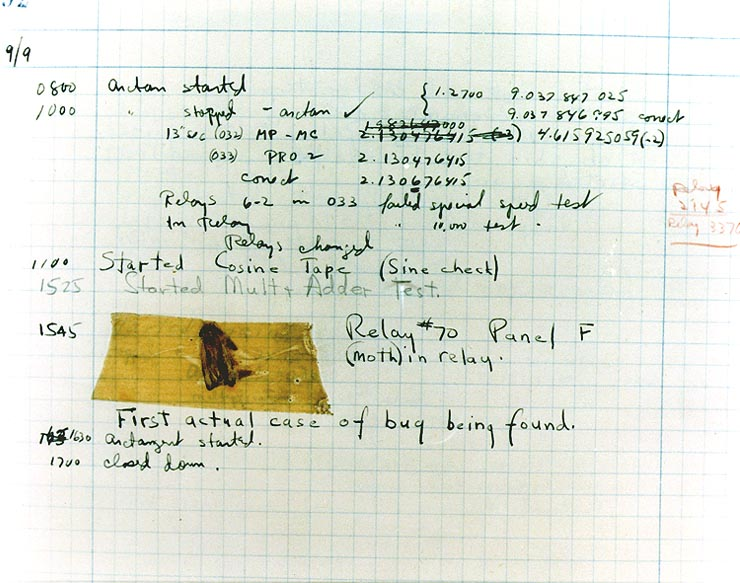
\includegraphics[width=0.6\textwidth]{first-bug.jpg}};
        \onslide<2->
        \node[anchor=south west, opacity=0.2] at (0,-36ex) {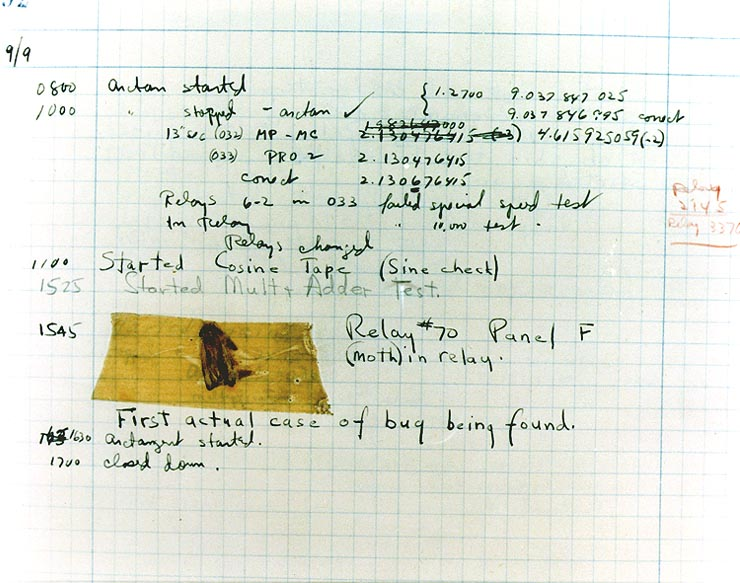
\includegraphics[width=0.6\textwidth]{first-bug.jpg}};
        \node[anchor=south west] at (0,-36ex) {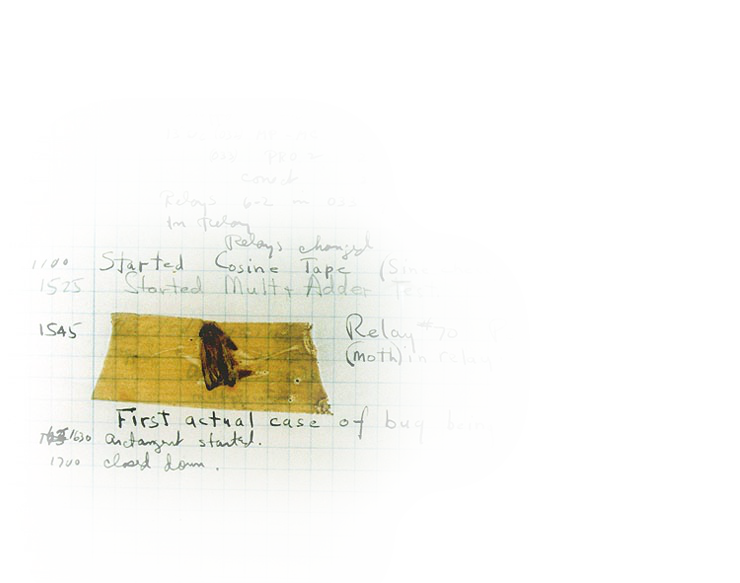
\includegraphics[width=0.6\textwidth]{first-bug.png}};
        \onslide<1->
    \end{tikzpicture}
    \pause  
    \tikz[overlay]\node[rotate=-6] at (60ex,10ex) {
\includegraphics[width=0.25\textwidth]{wikipedia.png}};
    In 1946, when \textbf{[Grace] Hopper} was released from active duty, she joined the Harvard Faculty at the Computation Laboratory where she continued her work on the Mark II and Mark III. Operators traced an error in the Mark II to a moth trapped in a relay, coining the term bug. This bug was carefully removed and taped to the log book. Stemming from the first bug, today we call errors or glitches in a program a bug.
\end{frame}

\begin{frame}
    \frametitle{Does it happen?}
    \tikz[overlay]\node[rotate=-6] at (60ex,9ex) {
\includegraphics[width=0.23\textwidth]{Stroustrup_PPP.jpg}};
    \begin{itemize}[<+->]
        \item When we write programs, errors are natural and unavoidable.
        \item \textit{The last bug} is a programmers’ joke.
        \item By the time we might have, we are busy modifying the program for some new use.
    \end{itemize}
\end{frame}

\begin{frame}
    \frametitle{Why does it happen?}
    \tikz[overlay]\node[rotate=-6] at (60ex,4ex) {
\includegraphics[width=0.25\textwidth]{Stroustrup_PPP.jpg}};
    \begin{itemize}[<+->]
        \item poor specification
        \item incomplete programs
        \item unexpected inputs \& arguments
        \item unexpected state
        \item logical errors
    \end{itemize}
    \onslide<+->Errors are always more common when you are tired or rushed.
\end{frame}

\begin{frame}
    \frametitle{Does it matter?}
    \begin{itemize}[<+->]
        \item Therac-25 Radiation Therapy Machine \small$\longrightarrow$ overdosed six people
        \item Northeast Blackout of 2003 \small$\longrightarrow$ 55,000,000 people affected 
        \item Pentium FDIV Bug \small$\longrightarrow$ \$475,000,000 cost
        \item NASA Mariner 1 Destruction \small$\longrightarrow$ \$18,500,000 cost
        \item Year 2000 Problem
    \end{itemize}
\end{frame}

\begin{frame}
    \frametitle{What should we do?}
    \begin{itemize}[<+->]
        \item debug
        \item test
        \item formal verification
        \item design for test \& debug\onslide<+->, write clean codes
    \end{itemize}
\end{frame}

\begin{frame}
    \frametitle{How far should we go?}
    \tikz[overlay]\node[rotate=-6] at (60ex,7ex) {
\includegraphics[width=0.25\textwidth]{Stroustrup_PPP.jpg}};
    \begin{itemize}[<+->]
        \item Eliminating \textit{all} errors?
        \item What about kicking out the power cord from the computer while it executed the program?
        \item What about data lose in safety-critical systems such as a medical monitoring program or the control program for a telephone switch?
    \end{itemize}
\end{frame}

\subsection{Debug}

\begin{frame}
    \frametitle{Debugging is hard}
    \begin{quote}
        Everyone knows that debugging is twice as hard as writing a program in the first place.

        \hfill\scriptsize ---~Brian Kernighan
    \end{quote}
\end{frame}

\begin{frame}
    \frametitle{Debugging is really hard}
    \begin{figure}
        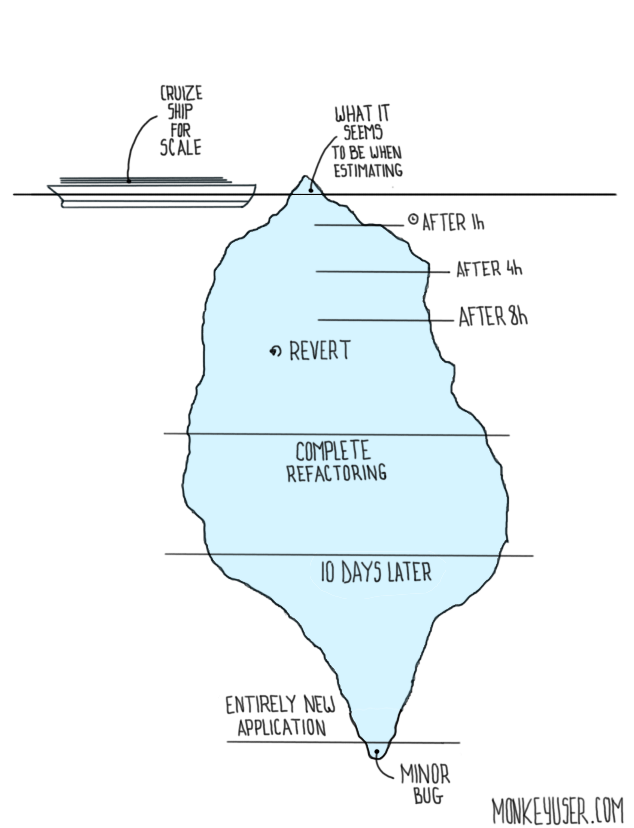
\includegraphics[height=0.8\textheight]{minor-bug.png}
    \end{figure}
\end{frame}

\begin{frame}
    \frametitle{Bugs are so complex}
    \begin{figure}
        
\includegraphics[height=0.8\textheight]{root-cause.png}
    \end{figure}
\end{frame}
